\section{Preliminaries}
\label{Prelims}

\subsection{Notation}

First we introduce notation for expressing graph metrics. This notation will also be used throughout the paper. % TODO - GET RID OF SECOND LINE?

\begin{definition}
	Complement Set

	\noindent
	Given a graph $G = (V, E)$, for a set of vertices $S \subseteq V$ we define the complement set $\comp{S} = V \setminus S$
\end{definition}

\begin{definition}
	Cut Set

	\noindent
	Given a graph $G = (V, E)$, for a set of vertices $S \subseteq V$ we define the cut set $ E(S, \comp{S}) = \left\{\{u, v\} \in E \mid u \in S, v \in \comp{S} \right\}.$
\end{definition}

\begin{definition}
	Degree of a vertex

	\noindent
	Given a graph $G = (V, E)$, let $d_v$ be the number of neighbouring nodes $v$ is adjacent to, i.e. $$
		d_v = |\left\{ e \in E : v \in e \right\}|
	$$
\end{definition}

\begin{definition}
	Volume of a vertex set

	\noindent
	Given a graph $G = (V, E)$ with $S \subseteq V$, let 
	$$
		\text{vol}(S) = \sum_{v \in S} d_v
	$$
\end{definition}

% TODO: Explain Implications of Cut set defn?

\subsection{Graph Metrics}\label{subsect:graphMetrics}

\begin{definition}
	Conductance of a graph $G = (V, E)$
	$$
		\Phi(G) = \min_{\emptyset \neq S \subset V} \frac{|E(S, \comp{S})|}{\min\{\text{vol}(S), \text{vol}(\comp{S})\}}
	$$
\end{definition}

\begin{definition}
	Diligence of a cut $ E(S, \comp{S}) $
	$$
		\rho(S) = \comp{d}(S) \min_{\{u, v\} \in E(S, \comp{S}) } \left\{ \max \left\{ \frac{1}{d_u},\frac{1}{d_v} \right\} \right\}
	$$ 
	where $\comp{d}(S) := \frac{\sum_{v \in S} d_v}{|S|}$ is the average degree of the vertices in $S$
\end{definition}

\begin{definition} % TODO: This definition doesn't include size bounds on S
	Diligence of a graph $G$
	$$
		\rho(G) = \min_{0 < \text{vol}(S) \leq \frac{\text{vol}(V)}{2}} \rho(S) 
	$$
\end{definition}

\subsection{Introducing Dynamic Networks}

Here we formally define the Dynamic Network structure rumours will spread on.

\begin{definition}
	Dynamic Network

	\noindent
	A dynamic network is a sequence of graphs $\mathcal{G} = (G_t)_{t \in \mathbb{N}}$ indexed by an integer time $t$. All the graphs in the sequence have the same vertex set at each time step, but the edge set may vary, i.e.  $G_t = (V, E_t)$ where $E_t$ is some edge set on $V$.
\end{definition}

$G_t$ represents the topology of the network at the discrete time step $t$. However, asynchronous rumour spreading algorithms operate in continuous time, so we need to define the topology of the network at non-integer times. To represent the state of the network at any non-negative continuous time $\gamma \in \mathbb{R}_+$, we say that the current network topology $G_\gamma$ := $G_{\floor\gamma}$. Thus, for any time $\gamma \in [t, t + 1)$ the network topology is fixed to $G_t$. This corresponds to allowing the network topology change at integer time steps only.

% TODO: Segway

\begin{definition}
	Vertex degree at time $\gamma \in \mathbb{R}_+ $ 

	\noindent
	For a Dynamic Network $\mathcal{G}$ on a vertex set $V$, $d_v(\gamma)$ is the degree of a vertex $v \in V$ at time $\gamma$, i.e. the degree of $v$ in $G_\gamma$
\end{definition}


\subsection{Review of Poisson Processes}

In this subsection we review some key properties of the Poisson process, which will be needed to specify the first asynchronous rumour spread algorithm.

The Poisson process ...
%%% COUNTING PROCCESS START
\begin{definition}
	Counting Process

	\noindent
	A counting process $\left\{ N(t), t \geq 0 \right\}$ is a right-continuous non-decreasing random function $N$ from non-negative reals to non-negative integers such that $N(0) = 0$.
\end{definition}

\begin{figure}[h]
	\centering
	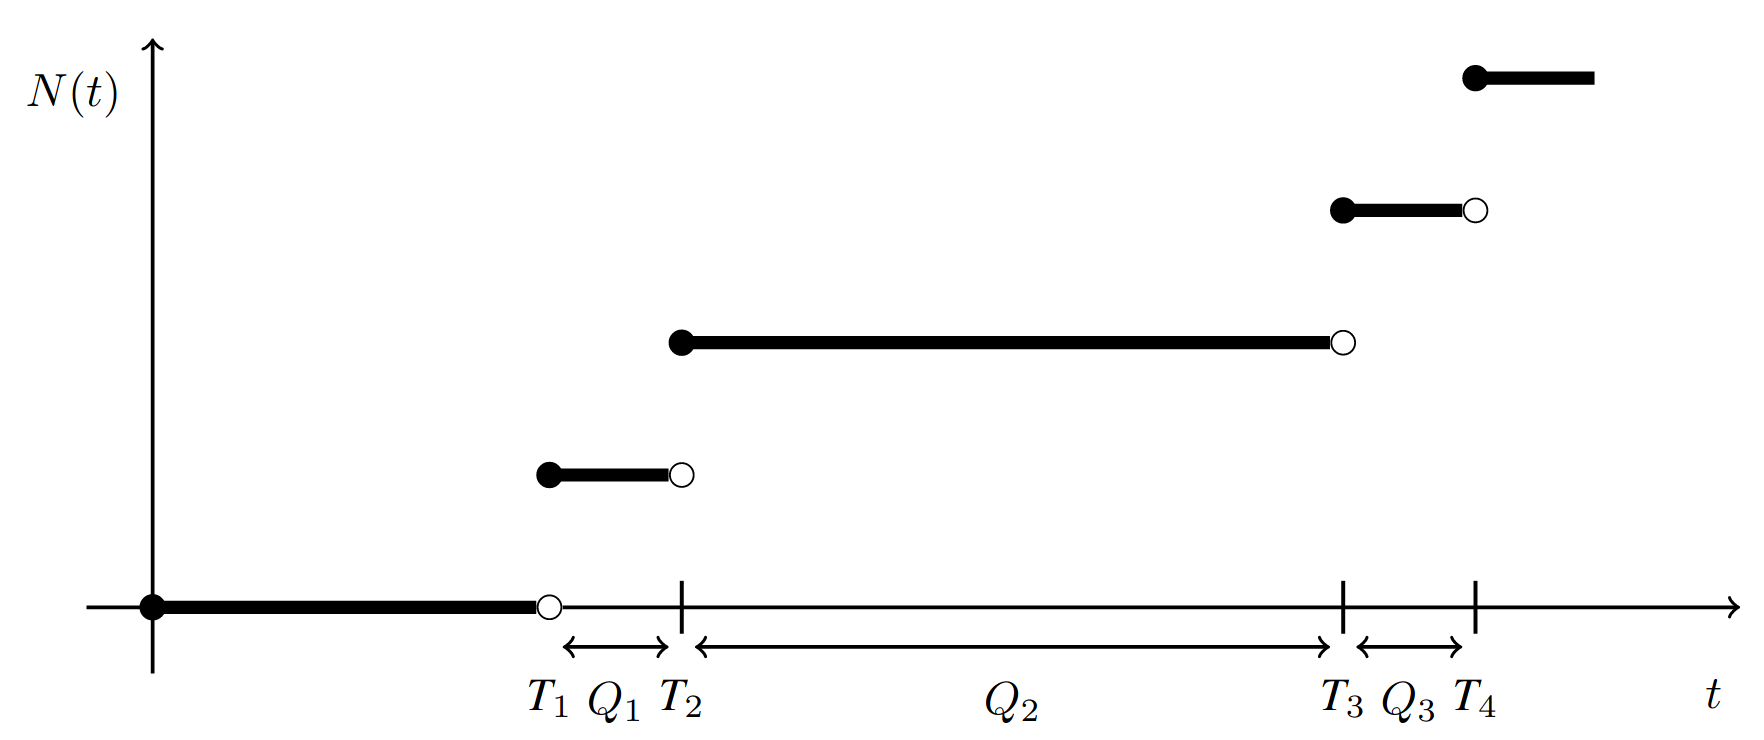
\includegraphics[width=\textwidth]{./figures/poisson_process_example.png}
	\caption{Example of a counting process from \cite{countingProcessFigure}}
	\label{fig:poissonProcessExample}
\end{figure}

% TODO: Discuss figure

We interpret the function $N$ as counting the number of occurrences of an event, where $N(t)$ represents the number of events that have occurred up to and including time $t$. We refer to the occurrences of events as "arrivals".  Since $N$ is right-continuous, $N$ increments exactly at the times of arrivals. For example, if $a^\text{th}$ arrival happens at time $t$, then $N(t) = a$, $\lim_{x \downarrow t} = a$, and $\lim_{x \uparrow t} = a - 1$. Note that the nuumber arrivals in the interval $(s, t]$ is represented by the random variable $N(t) - N(s)$. 
%%% COUNTING PROCCESS END

The Poission process is a type of counting process that satisfies additional conditions. 

\begin{definition}
	Homogenous Poisson Process

	\noindent
	A Homogeneous Poisson process ${N(t), t \geq 0}$ with rate $\lambda > 0$ is a counting process such that
	\begin{enumerate}
		\item $N(t)$ has independent increments
		\item for all $t \geq 0$, 
		\begin{align*}
			\mathbb{P}(N(t + \delta) - N(t) = 0) &= 1 - \lambda\delta + o(\delta) \\
			\mathbb{P}(N(t + \delta) - N(t) = 1) &= \lambda\delta + o(\delta) \\
			\mathbb{P}(N(t + \delta) - N(t) > 1) &= o(\delta)
		\end{align*}
		\item $N(0) = 0$
	\end{enumerate}
\end{definition}

The Poisson process can be used to model situations where % TODO: FINISH

%TODO: NEED SUPERPOISITION AND EQUIVALENCE WITH EXPONENTIAL

\subsection{Inhomogeneous Poisson Processes}

In this section we introduce an extension of the Poisson process which will be needed for the proof of Theorem \ref{theorem:AsyncUpperBound}.

\begin{definition}
	Inhomogeneous Poisson process

	\noindent
	An inhomogeneous Poisson process ${N(t), t \geq 0}$ with rate function $\lambda(t) > 0$ is a counting process such that
	\begin{enumerate}
		\item $N(t)$ has independent increments
		\item for all $t \geq 0$, 
		\begin{align*}
			\mathbb{P}(N(t + \delta) - N(t) = 0) &= 1 - \lambda(t)\delta + o(\delta) \\
			\mathbb{P}(N(t + \delta) - N(t) = 1) &= \lambda(t)\delta + o(\delta) \\
			\mathbb{P}(N(t + \delta) - N(t) > 1) &= o(\delta)
		\end{align*}
		\item $N(0) = 0$
	\end{enumerate}
\end{definition}

In this process the rate of arrivals can vary over time. This property is reflected in part 2 of the definition: the probability that a single arrival occurs in a small interval $(t, t+\delta]$ is proportional to a time-dependent rate $\lambda(t)$. The greater flexibility of the inhomogeneous process allows it to model a wider variety of stochastic processes than the homogeneous process. In the proof of Theorem \ref{theorem:AsyncUpperBound}, we will see one such process.

We now prove a property of inhomogeneous Poisson process which will be essential for Theorem \ref{theorem:AsyncUpperBound}. 

\begin{theorem}
	Let $\{N(t), t \geq 0\}$ be an inhomogeneous Poisson process with rate function $\lambda(t)$. Then $N(t)$ has a Poisson distribution with mean
	$$
		\Lambda(t) = \int_0^t \lambda(x) dx
	$$
\end{theorem}

\begin{proof}
	For brevity, let $p_n(t)$ denote $\mathbb{P}(N(t) = n)$. Let $\delta$ be small.
	First we derive an equation that the PDF of $N(t)$ must satisfy.
	We note that by the law of total probability
	$$
		p_n(t+\delta) = \sum_{k=0}^n \mathbb{P}(N(t) = k \cap N(t + \delta) - N(t) = n - k) 
	$$
	Since $N$ has independent increments, $N(t)$ and $N(t + \delta) - N(t)$ are independent, hence we have that the previous expression simplifies to
	$$
		\sum_{k=0}^n p_k(t) \mathbb{P}(N(t + \delta) - N(t) = n - k) 
	$$
	We now split the summation into three parts and evaluate each separately using the definition of the inhomogeneous Poisson process.
	\begin{align*}
		&\sum_{k=0}^{n-2} p_k(t) \mathbb{P}(N(t + \delta) - N(t) = n - k) \\ 
		&+ p_{n-1}(t) \mathbb{P}(N(t + \delta) - N(t) = 1) \\
		&+ p_n(t) \mathbb{P}(N(t + \delta) - N(t) = 0) 
	\end{align*}
	Recall that
	$$
		\mathbb{P}(N(t + \delta) - N(t) = k) 
		= o(\delta)
	$$
	for every $k > 1$, hence the first term is $o(\delta)$ as $\sum_{k=0}^{n-2} p_k(t)$ is at most 1 and constant with respect to $\delta$.  
	By applying the other interval conditions, we obtain that
	$$
		p_n(t+\delta) = p_n(t)(1-\lambda(t)\delta) + p_{n-1}(t)\lambda(t)\delta + o(\delta)
	$$
	where we have collected the $o(\delta)$ terms.
	Thus, it follows that
	\begin{align*}
		\frac{d}{dt} p_n(t) 
		&= \lim_{\delta \to 0} \frac{p_n(t+\delta) - p_n(t)}{\delta} \\
		&= \lim_{\delta \to 0} \left( -\lambda(t)p_n(t) + \lambda(t)p_{n-1}(t) + \frac{o(\delta)}{\delta} \right)\\
		&= -\lambda(t)p_n(t) + \lambda(t)p_{n-1}(t)
	\end{align*}
	% TODO: Introduce little and big o-notation, little o(x) is any f(x) such that f(x)/x -> 0 as x -> 0
	Therefore the PDF of $N(t)$ must satisfy the above ODE. 
	We now show that the Poisson distribution with mean $\Lambda(t)$
	satisfies this equality. It is possible to derive the p.d.f from the equation using the integrating factor technique \cite{inhomoPoissonProof}, however instead we will verify that the Poisson distribution p.d.f is sufficient.
	Let $q_n(t)$ denote the Poisson p.d.f with mean $\Lambda(t)$, i.e.
	$$
		q_n(t)
		= e^{-\Lambda (t)}\frac{(\Lambda(t))^n}{n!}
	$$
	Using the product rule we find that 
	$$
		\frac{d}{dt} q_n(t) 
		= \frac{d}{dt} \left[ e^{-\Lambda (t)}\right] \frac{(\Lambda(t))^n}{n!} + e^{-\Lambda (t)} \frac{d}{dt} \left[ \frac{(\Lambda(t))^n}{n!} \right]
	$$
	To evaluate this expression, we compute the derivates. By the Fundamental Theorem of Calculus,
	$$
		\frac{d}{dt} e^{-\Lambda (t)} 
		= \frac{d}{dt} \left[ - \int_0^t \lambda(x) dx \right] e^{-\Lambda (t)} 
		= - \lambda(t)  e^{-\Lambda (t)}
	$$
	and, 
	$$
		\frac{d}{dt} \left[ \frac{(\Lambda(t))^n}{n!} \right] 
		= \frac{d}{dt} \left[ \int_0^t \lambda(x) dx \right] \frac{(\Lambda(t))^{n-1}}{(n-1)!}
		= \lambda(t) \frac{(\Lambda(t))^{n-1}}{(n-1)!}
	$$
	Hence,
	\begin{align*}
		\frac{d}{dt} q_n(t) 
		&= - \lambda(t) e^{-\Lambda (t)} \frac{(\Lambda(t))^n}{n!} + \lambda(t) e^{-\Lambda (t)} \frac{(\Lambda(t))^{n-1}}{(n-1)!} \\
		&= -\lambda(t)q_n(t) + \lambda(t)q_{n-1}(t)
	\end{align*}
	% TODO: WHAT DOES ABOVE MEAN? - Solved equation
	% TODO: p = q + c, Unqiueness by some inital condtion
	Initial conditions
	$
		p_0(0) = 1, p_k(0) = 0, k > 0 
	$
\end{proof}

% TODO: Equivalent formulations + proofs
% TODO: Introduce indepdendent increments


\subsection{Order statistics of exponential random variables}



\subsection{Stochastic Domination}
Coupling proof of stochastic domination of poisson 



\begin{definition}
	First-order Stochastic Domination

	\noindent
	Let $X$ and $Y$ be real random variables. $Y$ has a first-order stochastic dominance over $X$, denoted by $X \preceq Y$, if for all $x \in R$, 
	$$
		\mathbb{P}(Y \geq x) \geq \mathbb{P}(X \geq x)
	$$
\end{definition}

Stochastic domination specifies a partial order between random variables. However, not all random variables are comparable by stochastic domination. % TODO: Exmaples

% TODO: interpretation as partial order and PDFs vs CDFS (gamma figure) 
% Not always the case

\begin{figure}[h]
	\centering
	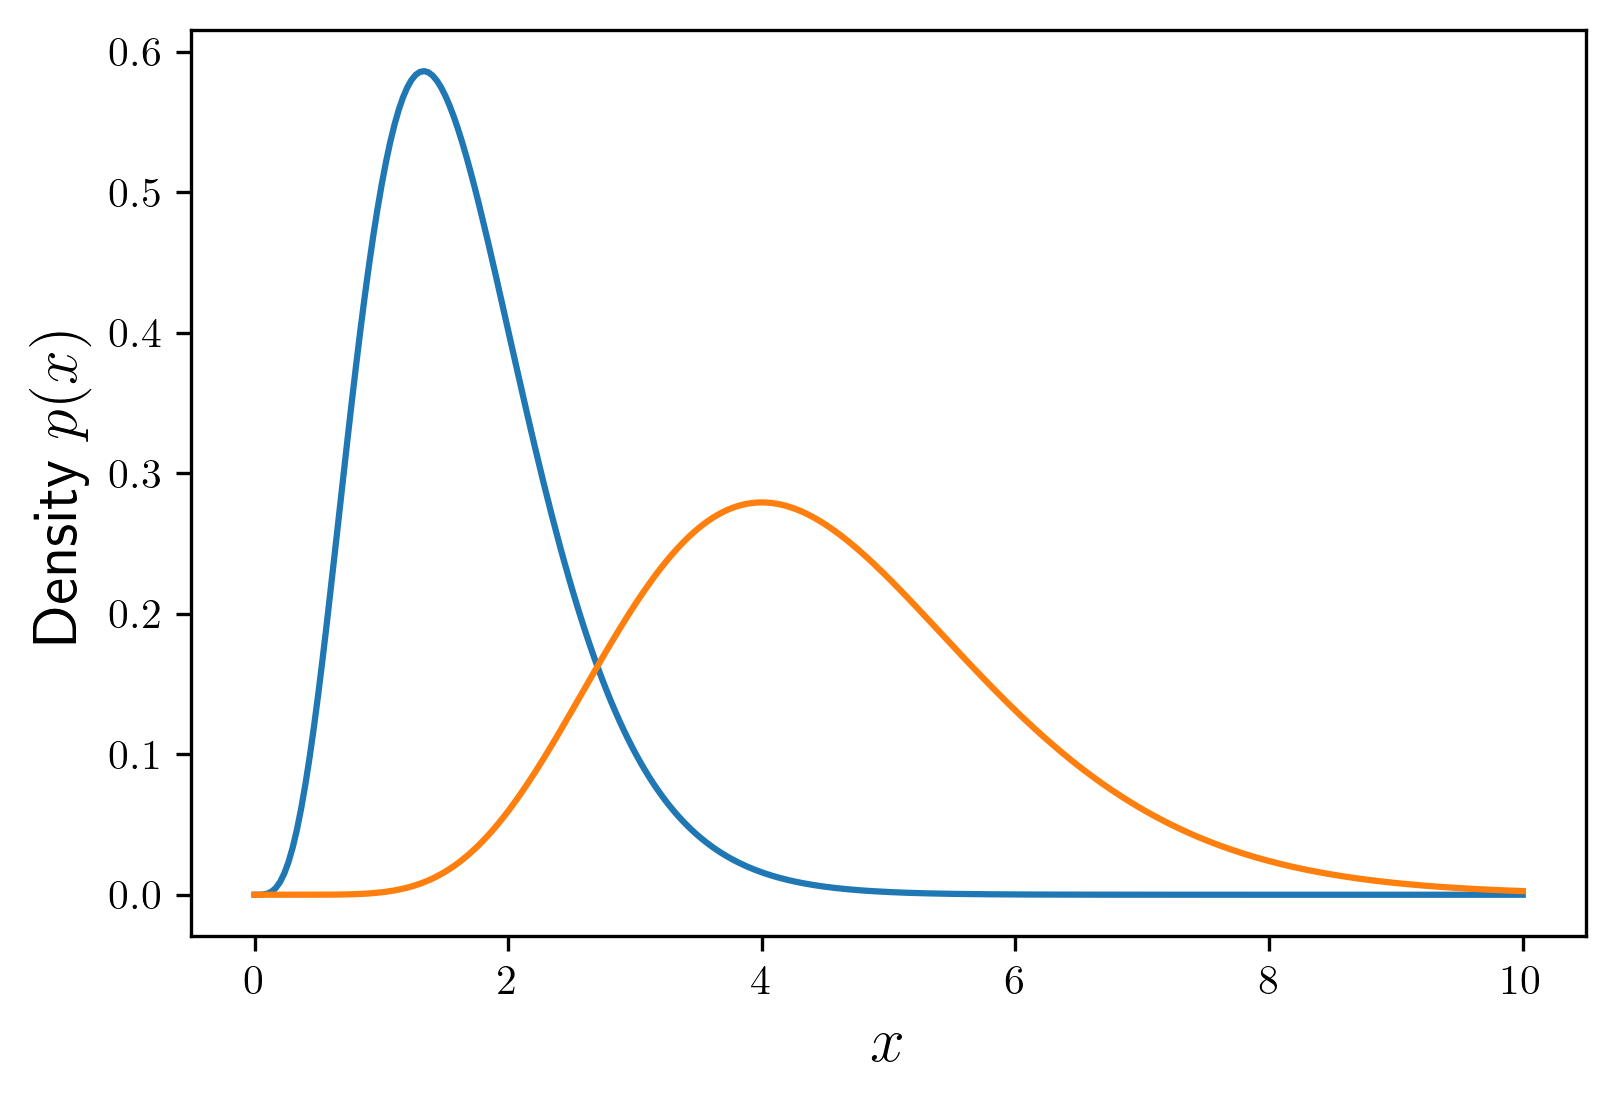
\includegraphics[width=0.8\textwidth]{./figures/stochastic_domination_pdf.png}
	\caption{Example of stochastic domination - PDFs}
	\label{fig:stochDomPDFs}
\end{figure}

Figure \ref{fig:stochDomPDFs} shows the probability density functions (PDFs) of two real random variables. In this example, the orange distribution stochastically dominates the blue distribution.

\begin{figure}[h]
	\centering
	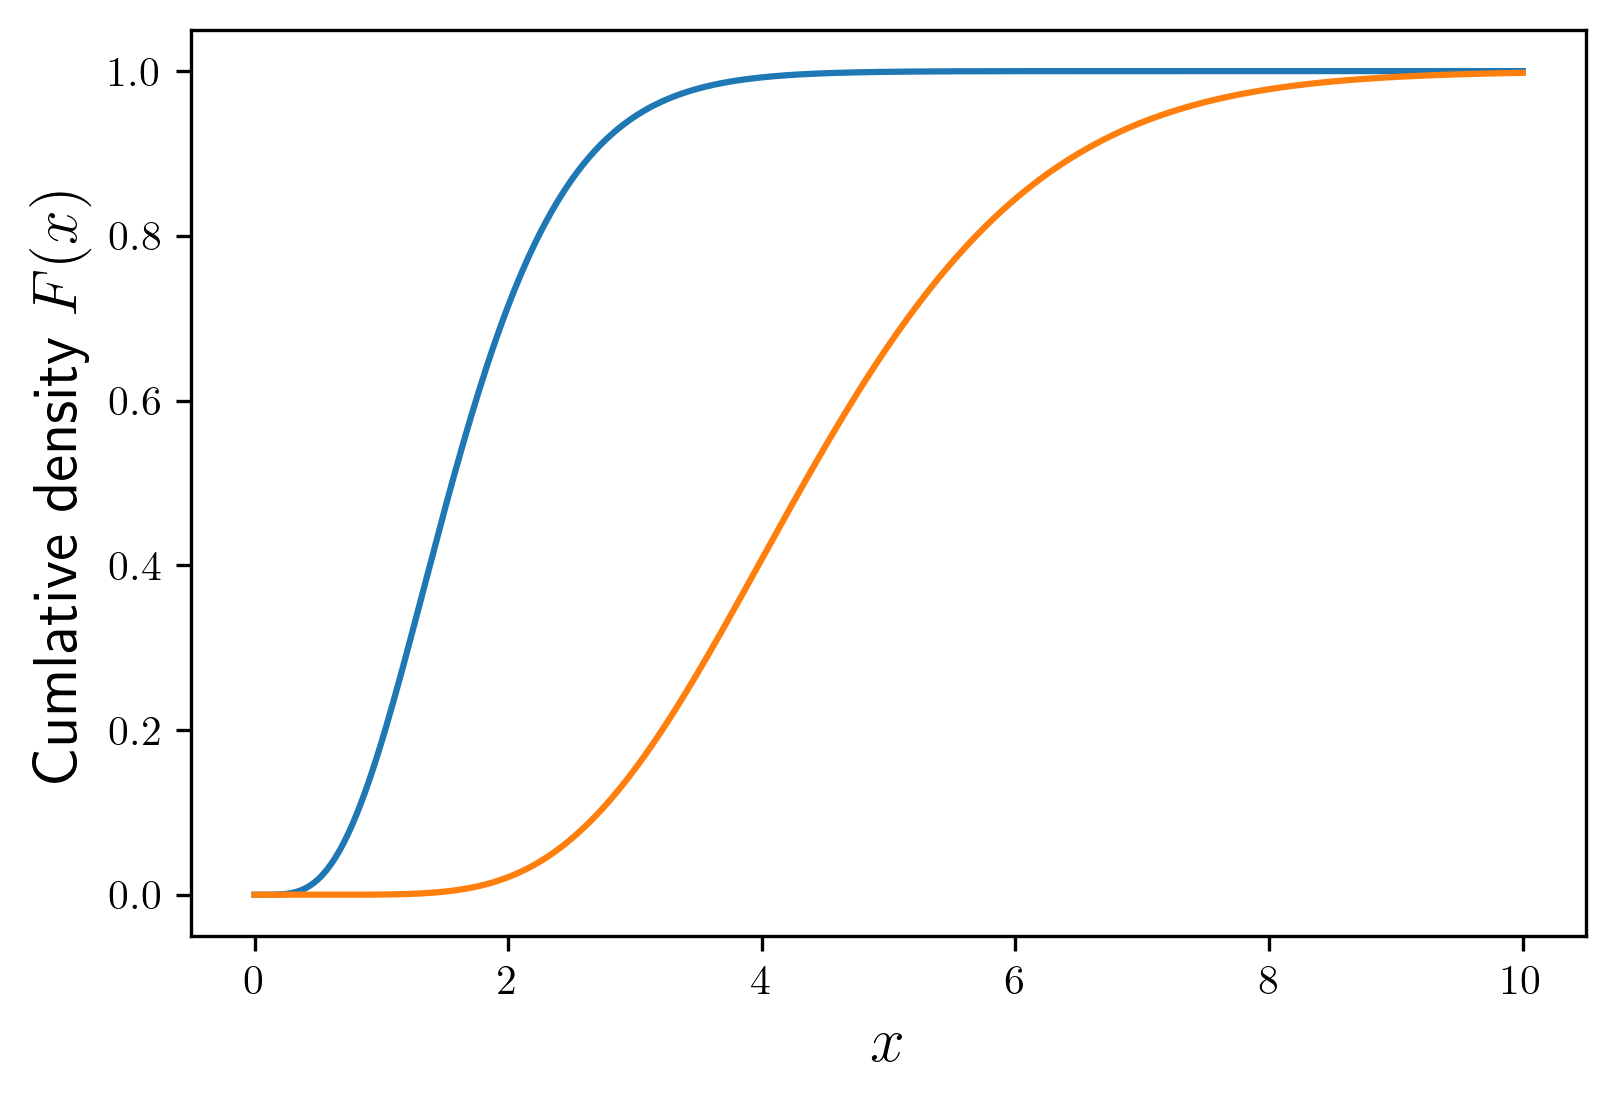
\includegraphics[width=0.8\textwidth]{./figures/stochastic_domination_cdf.png}
	\caption{Example of stochastic domination - CDFs}
	\label{fig:stochDomCDFs}
\end{figure}

Observe that $X \preceq Y$ if an only if $\mathbb{P}(Y \leq x) \leq \mathbb{P}(X \leq x)$. We recognise $\mathbb{P}(X \leq x)$ as the cumulative distribution function (CDF) of $X$. Hence, we verify this claim by computing the cumulative  distribution functions of the distributions in Figure \ref{fig:stochDomPDFs}, which are shown in Figure \ref{fig:stochDomCDFs}. Indeed, we see that the orange CDF is always below the blue CDF, hence the orange distribution does in fact dominate. % TODO: Reword, do we need this section?

For proofs in Sections \ref{section:AsyncUpperBound} and \ref{SyncFloodingSection} we need to establish stochastic dominance between pairs of Binomial random variables and Poisson random variables. To do this we use a technique called coupling. First we introduce the definition of a coupling.

\begin{definition} % TODO: Check definition
	Coupling

	\noindent
	A  coupling of the real random variables $X$ and $Y$ is a joint random variable $(\tilde{X}, \tilde{Y})$ such that the marginal distribution of $\tilde{X}$ is the same as $X$, and the marginal distribution of $\tilde{Y}$ is the same as $Y$.
\end{definition}

% TODO: when allowed different samples spaces, interpreation

Now we present a theorem which links couplings to first-order stochastic domination.

\begin{theorem}\label{theorem:couplingDomination}
	The real random variable $X$ is stochastically dominated by the real random variable $Y$ if and only if there exists a coupling $(\tilde{X}, \tilde{Y})$ of $X$ and $Y$ such that
	$$
		\mathbb{P}(\tilde{Y} \geq \tilde{X}) = 1
	$$
\end{theorem}

\begin{proof}
	We prove the forwards implication. Suppose there exists a coupling $(\tilde{X}, \tilde{Y})$ of $X$ and $Y$ such that $\mathbb{P}(\tilde{Y} \geq \tilde{X}) = 1$. Then for all $x \in \mathbb{R}$
	\begin{align*}
		\mathbb{P}(X \geq x) &= \mathbb{P}(\tilde{X} \geq x) & \text{since } \tilde{X} \stackrel{d}{=} X \\
		&\leq \mathbb{P}(\tilde{Y} \geq x) & \text{since with probability 1, } \tilde{Y} \geq \tilde{X} \\
		&= \mathbb{P}(Y \geq x) & \text{since } \tilde{Y} \stackrel{d}{=} Y 
	\end{align*}

	We omit the proof for the reverse implication as we only use the forwards implication. For the proof of the reverse implication, see \cite{coupling}.
\end{proof}

% TODO, introduce equal in distribution in coupling definition

Using Theorem \ref{theorem:couplingDomination}, we can establish stochastic domination between random variables by finding a coupling. We first show this technique	for pairs of Poisson random variables

\begin{theorem}
	Let $0 < \lambda < \mu$. If $X \sim \text{Poisson}(\lambda)$ and $Y \sim \text{Poisson}(\mu)$ are independent random variables, then $X \preceq Y$. 
\end{theorem}

\begin{proof}
	Let $\tilde{X} \sim \text{Poisson}(\lambda)$, $\tilde{Z} \sim \text{Poisson}(\mu - \lambda)$ be independent random variables. Hence, we have that $\tilde{Y} := \tilde{X} + \tilde{Z} \sim \text{Poisson}(\mu)$. Note that since $\tilde{Z} \geq 0$, the value taken by $\tilde{Y}$ is always at least the value taken by $\tilde{X}$. Since we have found a coupling $(\tilde{X}, \tilde{Y})$ of $X$ and $Y$ where $\mathbb{P}(\tilde{Y} \geq \tilde{X}) = 1$, by Theorem \ref{theorem:couplingDomination}, $X \preceq Y$.
\end{proof}

Now we use coupling to establish first-order stochastic dominance between pairs of binomial random variables.

\begin{theorem}
	Let $X \sim \text{Binomial}(n_1, p)$ and $Y \sim \text{Binomial}(n_2, p)$ be independent random variables with $n_1 < n_2$. Then $X$ is stochastically dominated by $Y$.
\end{theorem}

\begin{proof}
	Let $X_1, \dots, X_{n_2}$ be an iid sequence of Bernoulli random variables where $\mathbb{P}(X_i = 1) = p$. We observe that $\tilde{X} := \sum_{i=1}^{n_1} X_i \sim \text{Binomial}(n_1, p)$ and $\tilde{Y} := \sum_{i=1}^{n_2} X_i \sim \text{Binomial}(n_2, p)$. Since $X_i \geq 0$ for all $i$, and $\tilde{Y} = \tilde{X} + X_{n_1 + 1} + \dots + X_{n_2}$, we have that $\tilde{X} \leq \tilde{Y}$. Hence, by Theorem \ref{theorem:couplingDomination}, $X \preceq Y$.
\end{proof}

% TODO: Discuss implications for async rumour spreading - interpreting poission process as exponential clock, not interested in value of the process

